% HERE BE DRAGONS
% This is complicated because it is based on [SZM]'s 2012 Honours Thesis template, which in turn was based on a template written by a Physics Professor.
% ~50% of this isn't actually needed, but it's too much effort to clean it up.

\documentclass[a4paper,10pt,titlepage]{report}
%\linespread{1.3}
%\usepackage{setspace}
%\onehalfspacing 
 \parskip 10pt           % sets spacing between paragraphs
 %\renewcommand{\baselinestretch}{1.5} 	% Uncomment for 1.5 spacing between lines
 %\parindent 0pt		  % sets leading space for paragraphs


%\usepackage{natbib}
\usepackage{makeidx}
\usepackage{graphicx}
\usepackage{caption}
%\usepackage{subfigure}
\usepackage{rotating}
%\usepackage{lscape}
\usepackage{pdflscape} % Needed for landscaping - in pdf viewer
\usepackage{verbatim}
\usepackage{amsmath, amsthm,amssymb}
\usepackage{mathrsfs}
\usepackage{hyperref}

\usepackage{epstopdf}
\usepackage{float}
\usepackage[compact]{titlesec}
\titlespacing{\chapter}{0pt}{0pt}{0pt}
\titleformat{\chapter}
{\normalfont\LARGE\bfseries}{\thechapter.}{1em}{}

\usepackage[usenames,dvipsnames]{color}
\usepackage{listings} % For code snippets

\definecolor{darkgray}{rgb}{0.95,0.95,0.95}
\definecolor{darkred}{rgb}{0.75,0,0}
\definecolor{darkblue}{rgb}{0,0,0.75}
\definecolor{pink}{rgb}{1,0.5,0.5}
\lstset{language=Java}
\lstset{backgroundcolor=\color{darkgray}}
\lstset{numbers=left, numberstyle=\tiny, stepnumber=1, numbersep=5pt}
\lstset{keywordstyle=\color{darkred}\bfseries}
\lstset{commentstyle=\color{darkblue}}
%\lstset{stringsyle=\color{red}}
\lstset{showstringspaces=false}
\lstset{basicstyle=\small}



\newtheorem{theorem}{Theorem}[section]
\newtheorem{lemma}[theorem]{Lemma}
\theoremstyle{definition}\newtheorem{definition}[theorem]{Definition}
\newtheorem{proposition}[theorem]{Proposition}
\newtheorem{corollary}[theorem]{Corollary}
\newtheorem{example}{Example}
\theoremstyle{remark}\newtheorem*{remark}{Remark}

\newcommand{\Phid}[0]{\dot{\Phi}}
\newcommand{\Phib}[0]{\bar{\Phi}}

\newcommand{\de}[0]{\delta}
\newcommand{\deb}[0]{\bar{\delta}}

\newcommand{\that}[0]{\hat{\theta}}

\newcommand{\vect}[1]{\boldsymbol{#1}} % Draw a vector
\newcommand{\divg}[1]{\nabla \cdot #1} % divergence
\newcommand{\curl}[1]{\nabla \times #1} % curl
\newcommand{\grad}[1]{\nabla #1} %gradient
\newcommand{\pd}[3][ ]{\frac{\partial^{#1} #2}{\partial #3^{#1}}} %partial derivative
\newcommand{\der}[3][ ]{\frac{d^{#1} #2}{d #3^{#1}}} %full derivative
\newcommand{\phasor}[1]{\tilde{#1}} % make a phasor
\newcommand{\laplacian}[1]{\nabla^2 {#1}} % The laplacian operator



% Reference things in GitHub
\newcommand{\gitref}[2]{\href{https://github.com/UniversityComputerClub/FresherGuide/master/#1/#2}{  \textcolor{blue}{\emph{#2}}}}
% Refer to API commands
\newcommand{\api}[1]{  ``\textcolor{black}{\texttt{/api/#1}}''}
% Pun alert
\newcommand{\pun}[1]{\emph{#1}}
% Shell command
\newcommand{\shell}[1]{\texttt{#1}}
% Rants
\newcommand{\rant}[1]{\textsc{#1}}

% To make underscores printable without escaping them
\usepackage[T1]{fontenc}
\catcode`\_=12

% Refer to code (can change each one as needed)
\newcommand{\funct}[1]{  \texttt{#1}}
\newcommand{\var}[1]{  \texttt{#1}}
\newcommand{\type}[1]{  \texttt{#1}}
\newcommand{\code}[1]{  \texttt{#1}}


%\usepackage{endfloat}
%\nomarkersintext
\pagestyle{plain}
\topmargin -0.6true in
\textwidth 15true cm
\textheight 9.5true in
\oddsidemargin 0.25true in
\evensidemargin 0.25true in
\headsep 0.4true in

\usepackage{fancyheadings}
\pagestyle{fancy}
\addtolength{\headheight}{2.5pt}
\renewcommand{\chaptermark}[1]{\markboth{\thechapter~~#1}{}}
\renewcommand{\sectionmark}[1]{\markright{\thesection~~#1}{}}
\ifthenelse{\boolean{@twoside}}
{
        \rhead[\bfseries \rightmark]{\bfseries \thepage}
        \lhead[\bfseries \leftmark]{\bfseries \thepage}
        \addtolength{\headwidth}{\marginparsep}
        \addtolength{\headwidth}{\marginparwidth}
}{
        \lhead{\bfseries \leftmark}
        \rhead{\bfseries \thepage}
}
\cfoot{}

%---------------------------------------------------------
%---------------------------------------------------------
\begin{document}

\begin{titlepage}

% Suitably pretty title page is required.

\title{UCC::FresherGuide}
\author{The University Computer Club Inc. \\ \url{http://www.ucc.asn.au} \\ <\href{mailto:ucc@ucc.asn.au}{ucc@ucc.asn.au}>}

\date{January 2014}

\maketitle
\centering

\end{titlepage}
               % This is who you are

\pagenumbering{roman}
\newpage
%---------------------------------------------------------
% Do the table of Contents and lists of figures and tables
%---------------------------------------------------------
\linespread{0.8}
% Do we need these for a fresher guide?
\tableofcontents
%\listoffigures
\markboth{}{}
\linespread{1.0}
\newpage

\pagenumbering{arabic}
%---------------------------------------------------------
%---------------------------------------------------------
%Include the chapters!

\zchapter{Finding the Clubroom}\label{FindClubroom}

% Directions to the clubroom, ideally with non terrible maps. Most people don't ever find it :-(


\section{Maps}


\begin{figure}[H]
	\centering
	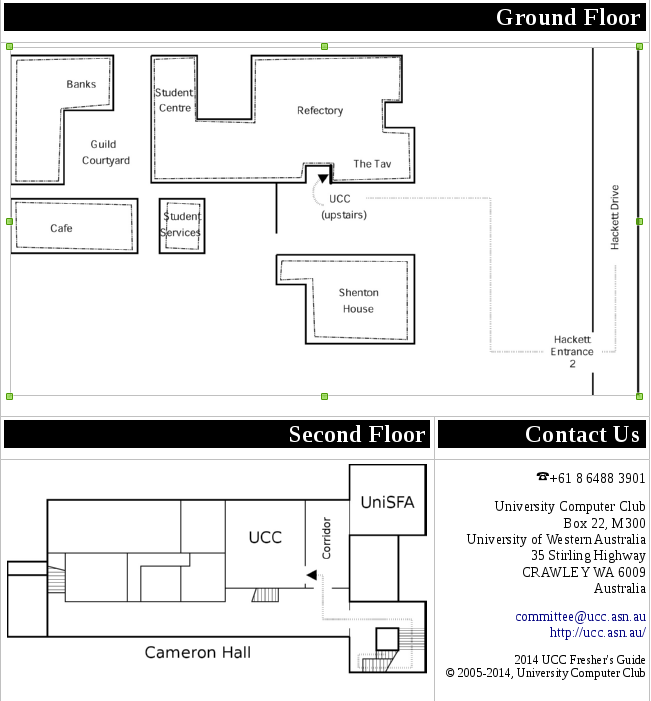
\includegraphics[width=1\textwidth]{figures/maps.png}
	\caption{Maps} 
	\label{maps.png}
\end{figure}

\pagebreak

\begin{mdframed}

\section{Directions}

\begin{enumerate}
	\item Starting from the carpark outside The Tav, follow the arrow on the aerial picture to get to the Cameron Hall door, then go up the stairs to the second floor and follow the bottom map.
	\item If you see a coke machine and a snack machine, you are in the right place. The UCC clubroom has lots of computers and a couple of couches.
	\item If you accidentally find yourself surrounded by books and a fridge, you're in UniSFA --- try the other door in that corridor.
\end{enumerate}

You can see if the clubroom is open online at \url{http://webcams.ucc.asn.au/}

\begin{figure}[H]
	\centering
	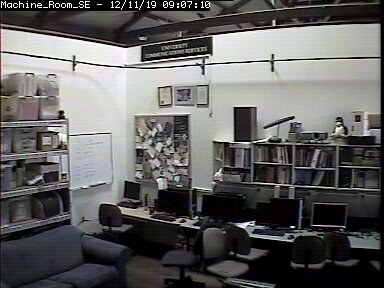
\includegraphics[width=0.7\textwidth]{figures/webcam2.jpg}
	\caption{This is what the clubroom looks like}
	\label{webcam2.jpg}
\end{figure}


\end{mdframed}
 % Chapter 1
\zchapter{Your Account}\label{SetupAccount}

% How to actually make an account. Most Freshers never do this :-(

%\begin{mdframed}

\section{Getting it}

\textsc{signing up at the O'Day stall does not give you access to all of UCC's services. You need to create an account at the UCC clubroom.}

Your UCC account is \emph{the} most important thing you can have as a member. In addition to providing a way for us to communicate with you, the account lets you log into any of our clubroom machines, as well as granting you access to our user servers, wireless network, online drink and snack machines, and more.

Once you're at the clubroom and ready to create an account, ask around for a Wheel or Committee member and have your membership sticker (we normally put it on your student card on O-Day) to set up your account. You'll need a user name and a password to memorise, but it's a pretty simple procedure once you've found the right person!


Now that you have an account, you can use it to log into any of our clubroom machines. If you want to log onto one of our servers, you'll need to use the SSH program. If you're having trouble, just ask someone in the clubroom --- we don't \pun{byte}!

Changing your UCC password can either be done by Ctrl-Alt-Del on a windows machine or using the command \shell{passwd} on a Linux/Unix machine.
Accessing the UCC WiFi network can be a bit tricky (particularly on Windows machines). Ask someone if you need help, or refer to \url{http://wiki.ucc.asn.au/Wifi}

%\end{mdframed}

%\begin{mdframed}

\section{SSH for Great Good}

SSH is a program that lets you remotely access UCC's servers. These can be used for almost anything (legal) you can imagine; programming, website hosting, file storage, IRC chatting, dispensing drinks, and many more things.

The easiest way to use SSH is from a Linux clubroom desktop. Simply open a "terminal" application, type "ssh ssh" and enter your password.

From a windows machine, open a program called "PuTTy" (or "KiTTy" on some machines). Enter the address "ssh" and click "Open".

Once you are logged in, a good way to start is running "irssi -c irc" and then typing "/join \#ucc". The interface of irssi takes some getting used to, but when combined with "screen" (ask someone for help) it is a powerful weapon for procrastination.

You don't have to be in the UCC clubroom to use SSH! Simply use "username@ssh.ucc.asn.au" as the address to connect to.

%\begin{figure}[H]
%	\centering
%	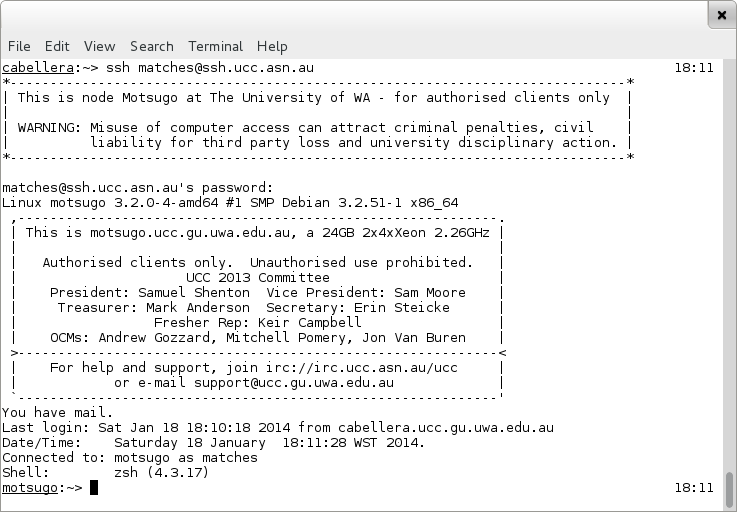
\includegraphics[width=1.0\textwidth]{figures/ssh.png}
%	\caption{SSH from Linux} 
%	\label{ssh.png}
%\end{figure}

%\begin{figure}[H]
%	\centering
%	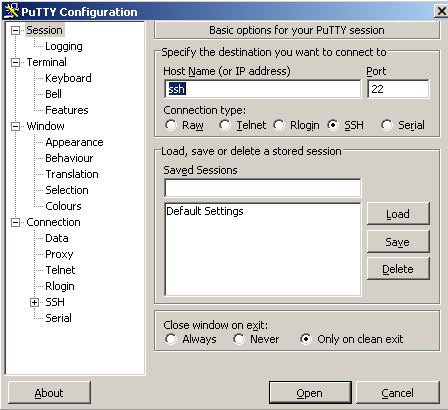
\includegraphics[width=0.5\textwidth]{figures/putty.png}
%	\caption{Use PuTTY to SSH. Just press "Open"} 
%	\label{putty.png}
%\end{figure}

%\end{mdframed}

\zchapter{Dispense 101}

% How to use Dispense.

\begin{mdframed}
\null
At the same time as you set up your account, you will also have your dispense account set up. Dispense is the program that allows users to store credit and purchase items from the coke/snack machines. Coke members can help you add credit to your dispense account. Call out for one in the clubroom if need be, there's always one around.


The easiest way to dispense a drink is probably the web interface (Figure \ref{webdispense.png}). Simply enter your username and password and then select a drink. 

Due to technical reasons, snacks cannot be dispensed using this interface. Getting a snack will involve typing a 5 digit User ID and a 4 digit PIN into the keypad. This allows you to dispense both drinks and snacks.

You can also use your Student Card or SmartRider as a log in device on the snack machine. To do so, log in to the Snack Machine and hold whichever card you want to use up to the card scanner (it's the thing with the blinking green light) and the card should auto- enroll. To log in using the card, simply hold the enrolled card up to the card scanner.


You can also access Dispense using the \shell{dispense} command. Dispense isn't installed on clubroom machines so you will have to use \shell{SSH} to access one of UCC's servers.

%\end{mdframed}

%\pagebreak

%\begin{mdframed}

\begin{figure}[H]
	\centering
	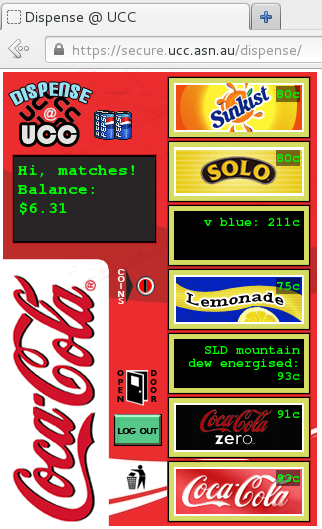
\includegraphics[width=0.3\textwidth]{figures/webdispense.png}
	\caption{\url{https://secure.ucc.asn.au/dispense}} 
	\label{webdispense.png}
\end{figure}
%
%\begin{figure}[H]
%	\centering
%	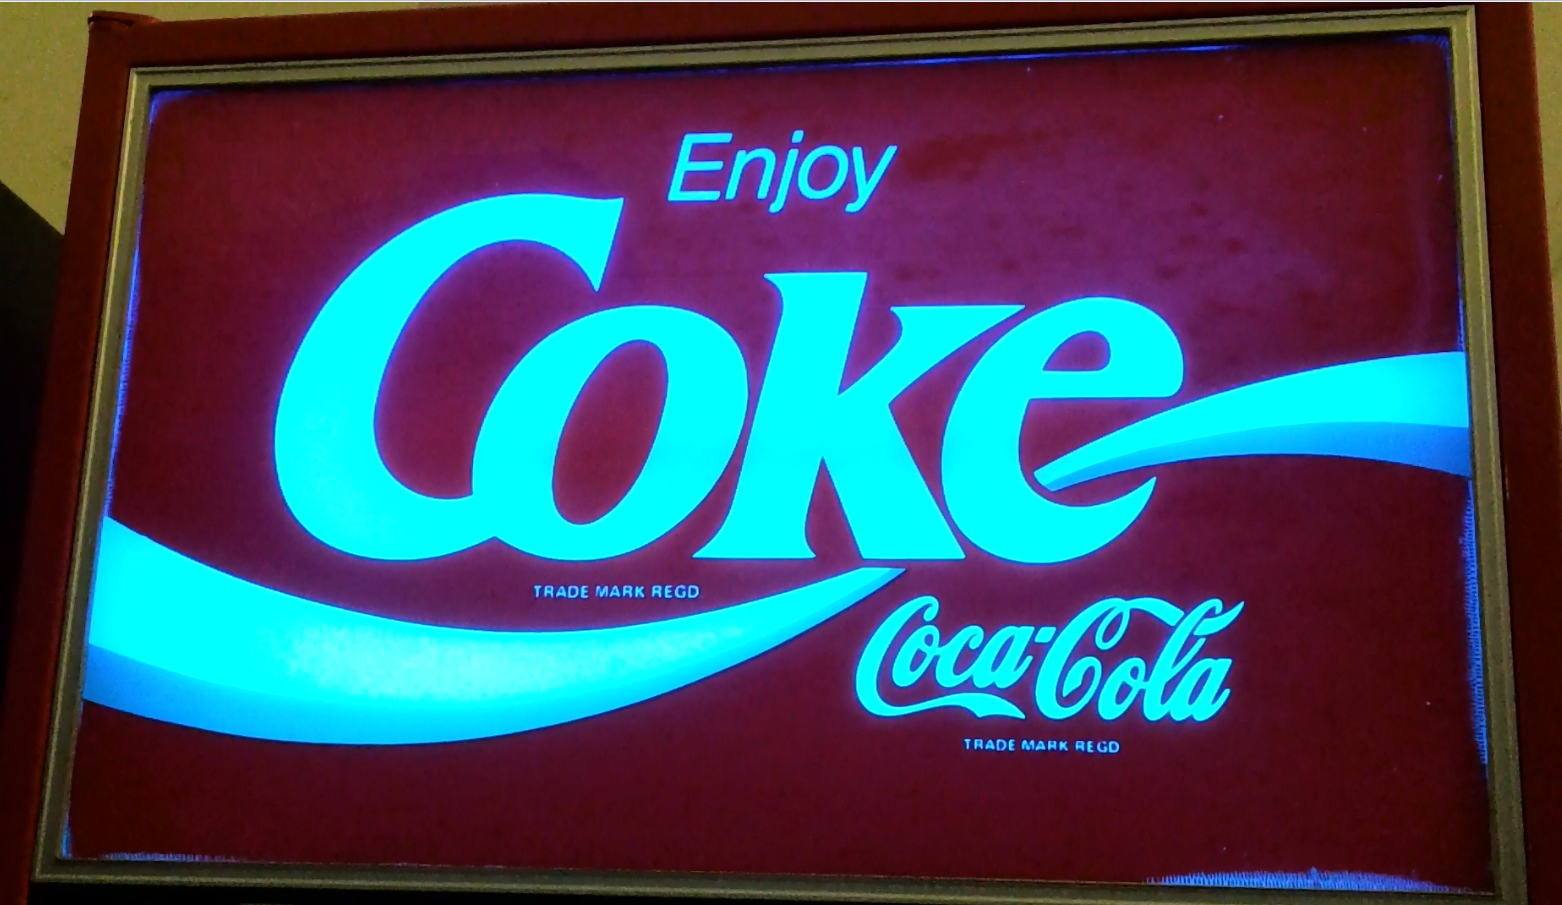
\includegraphics[width=0.75\textwidth]{figures/cokemachine.png}
%	\caption{Coke Machine}
%	\label{cokemachine.png}
%\end{figure}
%
\end{mdframed}

\zchapter{UCC::Groups}

% Explanation of the groups.
\newenvironment{uccgroup}[1] {
       \section{\textsc{\href{mailto:#1@ucc.asn.au}{#1@ucc.asn.au}}}
}

% Is this section a little elitist sounding, or is that just the entire group system? [SZM]
\begin{mdframed}
\null
The UCC committee delegates specific duties and responsibilities to other people in the club. These groups, traditionally modelled after UNIX groups, are referred to often.

You can see who's in each group online. Alternatively, if you're looking for a member of a certain group, shouting out "is there anyone here in group?" will sometimes get you an answer.


Membership of these groups entails a certain amount of trust. It is generally accepted that you will nominate yourself to the group once you feel you meet the requirements. Alternately, someone from the group may nominate you.

The requirements for applying for a group can be found by determined searching at \url{http://www.ucc.asn.au/infobase}.

% Don't really need to brand wheel like a cabal to new members. I mean, it is, but they don't need to know that for at least a few weeks.
%Members join Wheel by invite only, and will be asked to attend a Wheel Meeting, where they too will be taught the Secret Wheel Song.
%Do not despair if you're not made a Wheel member immediately. Sticking around and showing an interest through contribution is more important than just having the skills.


\end{mdframed}

\begin{uccgroup}{committee}
The Committee is appointed each year by the members (that's you) at the AGM. They handle the day-to-day running of the club, managing money, events and holding grumpy meetings each week, which members like yourself are welcome to attend.


The Fresher Rep is your voice on the Committee. Get to know them and let them know how incredibly happy you are! If you have problems, they'll always be ready to listen.

%\begin{mdframed}
Fresher Rep: <\href{mailto:fresher@ucc.asn.au}{fresher@ucc.asn.au}>
%\end{mdframed}
\end{uccgroup}

\begin{uccgroup}{door}
The Door group is responsible for the clubroom itself. Only a member of door group can unlock the clubroom and keep it open for members during the day. This means that if the only Door group member in the room has to leave, then everyone will have to leave until another Door group member arrives.
\end{uccgroup}

\begin{uccgroup}{wheel}
Wheel is in charge of maintaining the club's machines. They are the best people to see if you're having problems with the computers. Wheel maintains its own membership, but works hand in hand with Committee on issues relating to account policy. If you abuse your account, it will be locked by a Wheel member. The unlocking of accounts is at the discretion of Committee. Wheel have infrequent meetings, where they sing the secret wheel song. % THIS DOESN'T ACTUALLY HAPPEN
\end{uccgroup}

\begin{uccgroup}{coke}
The Coke group are the people to talk to if you want to add money to your dispense account (see the section on dispense). They can also credit your account for bad dispenses and other tasks related to dispense.
\end{uccgroup}

% Not even worth mentioning, really, it is all just wheel
\begin{uccgroup}{webmasters}

The Webmasters are charged with maintaining the UCC web presence. Becoming a Webmaster usually involves showing some interest in the UCC website. It shouldn't be too hard to get on this group.

 Please. Someone save us from the horror of doctype graham.
\end{uccgroup}

\begin{uccgroup}{winadmin}

The Winadmins group was created to give trusted members administrator access to the Windows desktop machines in the clubroom. Sprocket is the equivelant group for Linux desktop machines.

Sprocket/Winadmin is normally given on an adhoc basis to door members when they start to complain at wheel about things broken (``Someone should fix it you say? Excellent suggestion!'').

The committee might make a policy in 2014 I don't know.
\end{uccgroup}







\chapter{UCC::Clubroom}

%\begin{mdframed}
\null
The clubroom is usually open from about 9am until 11pm (staying later than this requires \emph{a good reason} and giving notice to UWA security). It is also sometimes open on weekends, and most days during university holidays. There is a map to the clubroom in Chapter \ref{FindClubroom}. If you want to check the clubroom is open and who is there, check out \url{http://webcam.ucc.asn.au}

The clubroom has a heap of desktop computers, a server room, a projects area with tool cupboard, and assorted storage areas for parts, books and components. These things are all there for members to use --- the locks on everything are to keep thieves out, so please don't be put off, and just ask if you need to get into something.

We don't have cleaners, so look after the clubroom! There is always a door group member in the room, \rant{and you will do what they damn well tell you to do as they are the ones who have to come to cleanups in their free time.} Of course, if you see something that needs doing such as cleaning up, feel free to do it!

\begin{figure}[H]
	\centering
	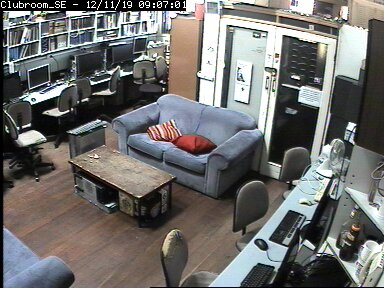
\includegraphics[width=0.5\textwidth]{figures/webcam.jpg}
	\caption{\url{http://webcam.ucc.asn.au}}
	\label{webcam.jpg}
\end{figure}


%\end{mdframed}
\chapter{Communication Technologies}

% Add Social Media?

\section{Mailing Lists}

UCC has a series of mailing lists that its members use to communicate. 
These include: 

UCC-Announce - An announcement list through which we let 
members know about Events and the like. You are automatically 
subscribed to this list when becoming a member. 

UCC - Having a party that you want to invite UCCans to? This is the 
list for you! Most UCCans subscribe to this list so it's a great 
source of information and discussion on both the club and general 
technical things. 

Committee - The list where committee matters are dealt with and circular 
discussions occur. If you are interested in the running of the club then 
you should subscribe to this list. 

Tech - Technical question? Suggestions or discussion around UCCs setup? 
The list used to discuss UCC's hardware and machines. 

If you want to subscribe to any of these lists, you can do so at 
\url{http://lists.ucc.gu.uwa.edu.au}

\section{IRC}

Without a doubt, the easiest way to waste time in or out of UCC 
is chatting on our Internet Relay Chat (IRC) server. 

You'll get to chat with some of the older members of the club who 
may not even be in Perth. Some of these old guard may seem a 
little grumpy or intimidating at first, but give them a chance, they 
are gold mines for information about the club and all things tech! 
We also have members from CASSA and ComSSA, clubs at other WA unis. 

You can connect with an IRC client to \texttt{irc://irc.ucc.asn.au:6667} 
and join the channel \texttt{\#ucc}, or with a web browser go to 
\url{http://irc.ucc.asn.au}

% ETC

%\newpage
%---------------------------------------------------------
\renewcommand{\bibname}{References}
\bibliography{references/refs}
\bibliographystyle{ieeetr}  
\addcontentsline{toc}{part}{References}
%---------------------------------------------------------

% Appendices
\appendix
\chapter*{Glossary}

Words and phrases that are (or were) useful around the club.

\begin{tabular}{ll}
	{\bf Term} & {\bf Meaning} \\
Dr ACC Murphy &
A Computer Called Murphy. Dr ACC Murphy is infamous around the UCC. He even receives mail! \\
BSD &
Berkeley Systems Distribution – a UNIX developed at Berkeley, now better known through the FreeBSD, NetBSD and OpenBSD UNIXes. musdea runs FreeBSD. \\
blog &
aka. weblog – sort of like a journal on the Internet (you don't have one?). Think of it as  a tumblr for grown-ups. Syndicated by a Planet. \\
Coke credit & 
If you gotta ask, you ain't got it! Coke credit is how people usually refer to money in your dispense account. \\
Coke Group &
The people who can put money (Coke credit) in your dispense account. \\
Debian &
a Linux distribution popular in the UCC due to its community nature. \\
DEC Terminal &
A dumb serial terminal, useful for plugging into the serial console on servers (possibly via a terminal server). Has a model number like vt100, vt200 or vt420. There's one in the corridor you can log into mussel and dispense drinks from. \\
dispense &
dispense started off as a way to dispense Cokes from the online Coke machine, and has since grown into the way UCCans think the world should do business. \\
Door Group &
the group of people charged with keep the room open, tidy and safe. \\
Firefox &
A web browser by the Mozilla Foundation, arguably the second-worst Internet browser – the worst is every other browser. \\
Flame &
Flame is the UCC's MUD (Multi-User Dungeon) and may or may not be haunted. \\
Fresher &
A new university student, usually also a first time UCC member. \\
Fresher Rep &
Fresher Committee member, usually chosen because they look like they'll make a good worker drone in the future. Represents the freshers at committee meetings, if they attend. \\
GNOME &
GNU Networked Object Model Environment – an open source desktop environment aimed primarily at UNIX computers. Quite popular in the past, before it removed all of the features people liked. \\
GNU &
GNU is Not Unix – a layer of libraries and utilities to implement a UNIX like operating system, commonly used on top of Linux. \\
Internet Explorer &
Just use Firefox. No, really. \\
IRC &
The lifeblood of UCCan communication. Internet Relay Chat lets you share news, stories and terrible puns with other members worldwide. \\
KDE &
The K Desktop Environment. A rival of GNOME which some members prefer. Contains a frankly scary number of features, and a memory footprint to match. \\
kernel &
The core of an operating system. All operating systems have a kernel, some popular ones include the Linux kernel and the Mach kernel. \\
LDAP &
Lightweight Directory Access Protocol: the black magic used for authentication at the UCC. \\
Linux &
the kernel (basis) of an open source UNIX operating system that has developed quite a following among computer scientists and engineers. \\
loft &
the area above the UCC that looks down into the UCC clubroom. LAN gaming and other activities take place up there. \\
machine room &
The UCC data centre. This is the small room with the glass doors that is located within the clubroom. All of our servers are kept in this room. It is locked when there is no one from Wheel around. \\
mailing list &
a way of communicating with a very large number of people via email. The UCC has several mailing lists of varying popularity. \\
Mozilla &
develop several open source web related products, such as Firefox and Thunderbird. \\
OCM &
Ordinary Committee Member – the worker drones of the UCC Committee, they do lots of work, for little reward. \\
Oligoboot &
boots more then one operating system (selectable when you boot). \\
OpenSolaris &
A UNIX developed by Sun Microsystems, and abandoned by Oracle. \\
NeXTStep &
An operating system developed by NeXT before they were bought out by Apple. Lots of NeXTStep is incorporated into Mac OS X. \\
open source &
A software ideology, where the source code to software (what is compiled into the program you run) is freely available. Also known as Free Software, exactly what makes a program open source is a good way to get into an argument. \\
Planet &
A web page that syndicates blogs. UCC has one at \url{http://planet.ucc.asn.au/} \\
Secret Wheel Song &
The song that is supposedly sung at the beginning of each Wheel meeting. \\ % Elitism alert...
SLA &
A Service Level Agreement. A document describing how reliable services are. UCC does not have one, and you should not ask Wheel members about it. \\
terminal server &
Sort of a router for serial ports, allows you to connect to one serial port from another. Usually connected to DEC Terminals, servers and dispense. (It can also refer to other sorts of servers which provide login sessions over the network). \\
theft book &
this is where you write down that you borrowed tools from UCC. It is not for borrowing books; you mail books@ucc.asn.au to do that. \\
TLA &
Three Letter Acronym – a way to refer to UCC members, often used in the minutes of meetings. Use the tla program or visit the UCC website to decode them. \\
Ubuntu &
A Linux distribution derived from Debian. Funded with space money. \\
UCCan &
someone who spends a lot of time in the UCC. Some UCCans pass their units. \\
Unifi &
The University wireless network. Available around campus where UCC's wireless is not. You need to be a student to access it though. \\
UniSFA &
the University Science Fiction Association, the ones down the hall. \\
VM &
A VM or Virtual Machine is a computer emulated on top of another computer. Many of the UCC's servers run inside VMs. The claim is that UCC's VMs are not a ``single point of  failure.`` That's the machine they are all running on (medico). \\
WAIX &
WA Internet eXchange – a group of ISPs and interested bodies who peer resources on the Internet for mutual benefit. \\
Wheel Group &
the group responsible for maintaining computers, accounts and services in UCC. \\
\end{tabular}

%\include{appendices/figures}

%---------------------------------------------------------

\end{document}

